\documentclass[a4paper,17pt]{extarticle}
\usepackage[utf8]{inputenc}
\usepackage{amsfonts}\usepackage{amssymb}\usepackage{amsmath}
\usepackage[top=2cm,left=1cm,right=1cm]{geometry}
\usepackage{tikz}
\usepackage{gensymb}\usepackage{ragged2e}\usepackage{blindtext}\usepackage{polynom} \usepackage{graphicx}

\begin{document}
\begin{center}
    MAT110 ASSIGNMENT 4 [SET-12]\\[6pt]
    NAME: ANIKA ISLAM \\[6pt]
    ID:21101298 \\[6pt]
    SECTION:08
\end{center}
\newpage
\begin{figure}[htbp!]
    \centering
    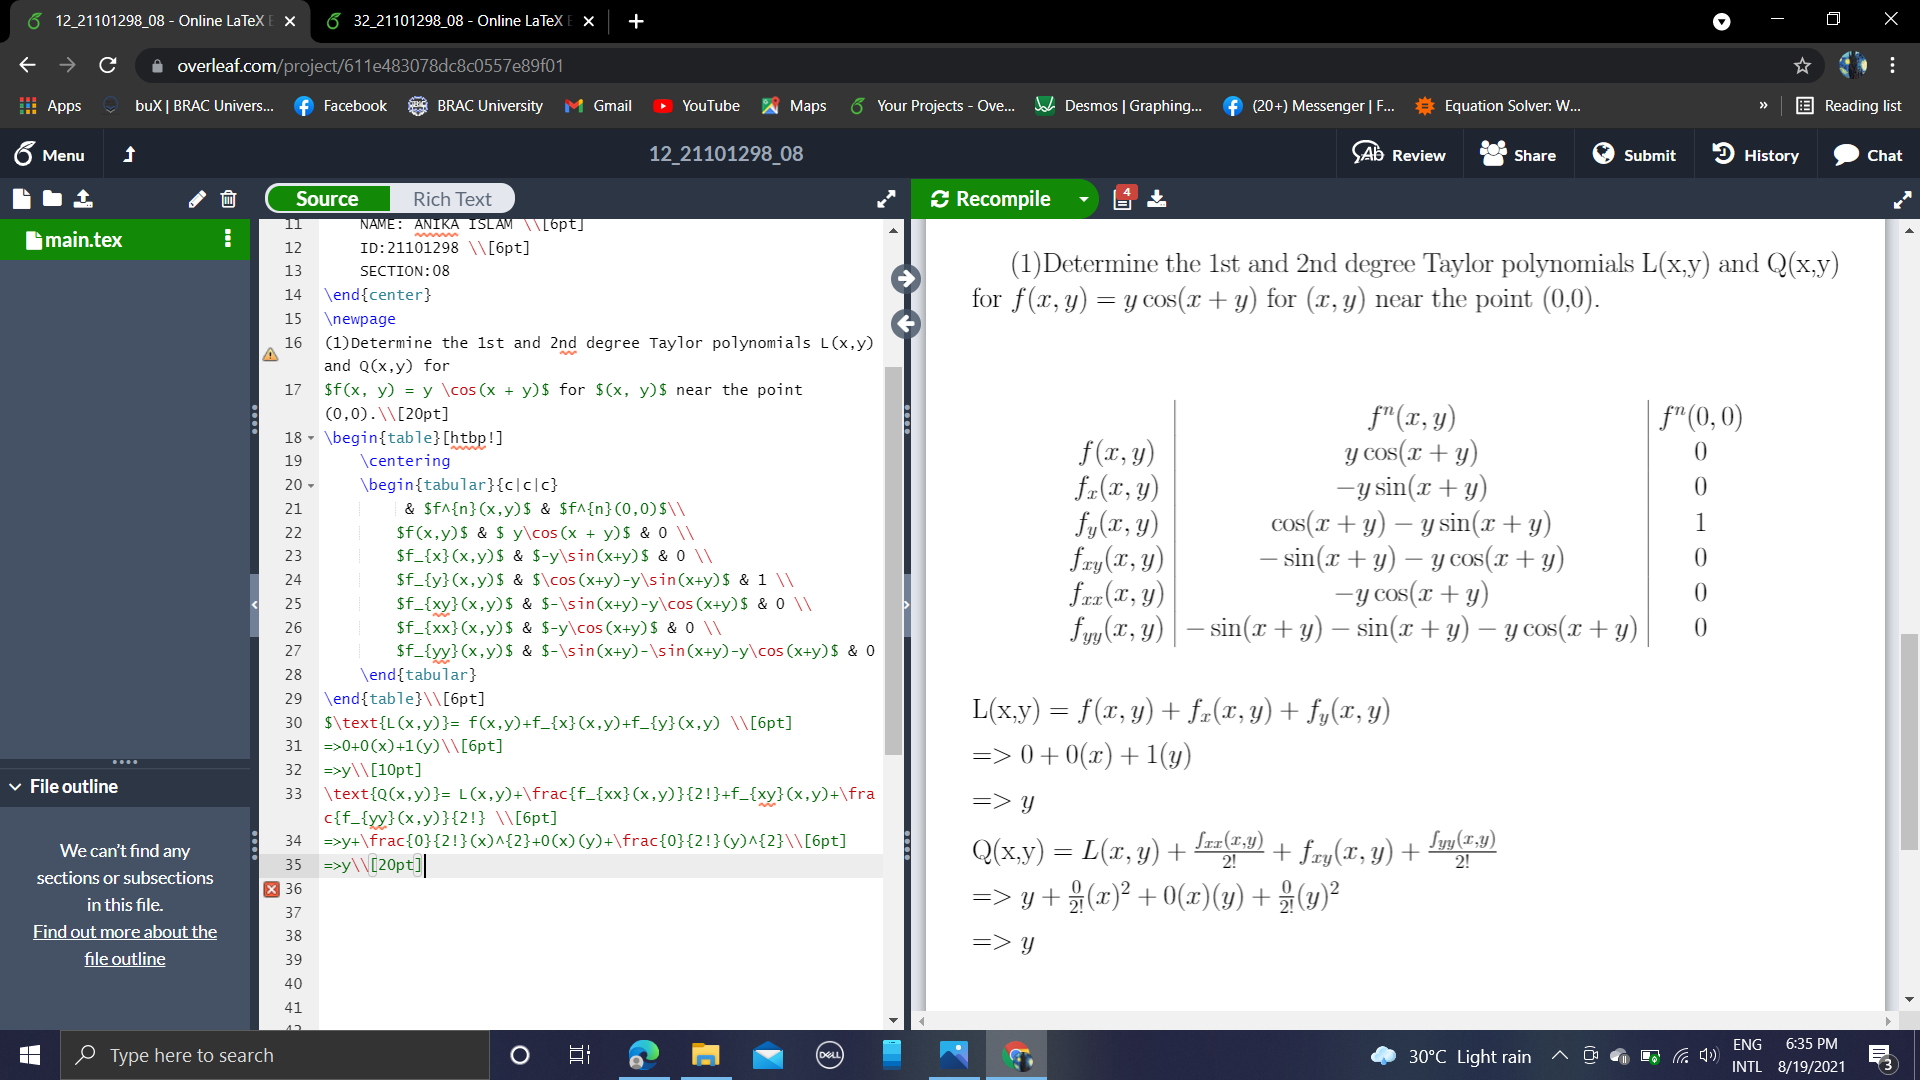
\includegraphics[width=1\linewidth]{SET 12.png}
    \caption{Screenshot of my Latex}
\end{figure}
\newpage
(1)Determine the 1st and 2nd degree Taylor polynomials L(x,y) and Q(x,y) for
$f(x, y) = y \cos(x + y)$ for $(x, y)$ near the point (0,0).\\[20pt]
\begin{table}[htbp!]
    \centering
    \begin{tabular}{c|c|c}
         & $f^{n}(x,y)$ & $f^{n}(0,0)$\\
        $f(x,y)$ & $ y\cos(x + y)$ & 0 \\
        $f_{x}(x,y)$ & $-y\sin(x+y)$ & 0 \\
        $f_{y}(x,y)$ & $\cos(x+y)-y\sin(x+y)$ & 1 \\
        $f_{xy}(x,y)$ & $-\sin(x+y)-y\cos(x+y)$ & 0 \\
        $f_{xx}(x,y)$ & $-y\cos(x+y)$ & 0 \\
        $f_{yy}(x,y)$ & $-\sin(x+y)-\sin(x+y)-y\cos(x+y)$ & 0
    \end{tabular}
\end{table}\\[6pt]
$\text{L(x,y)}= f(x,y)+f_{x}(x,y)+f_{y}(x,y) \\[6pt]
=>0+0(x)+1(y)\\[6pt]
=>y\\[10pt]
\text{Q(x,y)}= L(x,y)+\frac{f_{xx}(x,y)}{2!}+f_{xy}(x,y)+\frac{f_{yy}(x,y)}{2!} \\[6pt]
=>y+\frac{0}{2!}(x)^{2}+0(x)(y)+\frac{0}{2!}(y)^{2}\\[6pt]
=>y\\[20pt]$
\newpage
(2)Locate all relative maxima, relative minima and saddle points (if any) for
$f(x, y) =1-x^{2}-y^{2}$\\[20pt]
$f_{x}(x,y)=-2x\\[6pt]
f_{y}(x,y)=-2y\\[6pt]
\text{At critical points}, \\[6pt]
f_{x}(x,y)=0\\[6pt]
=>-2x=0\\[6pt]
=>x=0\\[6pt]
f_{y}(x,y)=0\\[6pt]
=>-2y=0\\[6pt]
=>y=0\\[6pt]
(0,0)\\[6pt]
f_{xx}(x,y)=-2\\[6pt]
f_{yy}(x,y)=-2\\[6pt]
f_{xy}(x,y)=0\\[6pt]
\text{At critical points},\\[6pt]
f_{xx}(x,y)=-2\\[6pt]
f_{yy}(x,y)=-2\\[6pt]
f_{xx}(x,y)f_{yy}(x,y)=(-2)(-2)=4\\[6pt]
f_{xx}(x,y)f_{yy}(x,y)>(f_{xy})^{2}\\[6pt]
=>4>0\\[6pt]
\text{Since} \ f_{xx}(x,y) \  \text{and} \ f_{yy}(x,y) < 0 , f_{xx}(x,y)f_{yy}(x,y)>(f_{xy})^{2} \ f(x,y) \ \text{has}\\ \text{relative maximum at } (0,0) \\[20pt]$
\newpage
(3)Find the unit vector that has the same direction as $v =< 4, 1, -3 >.$\\[20pt]
$|v|=\sqrt{(4)^{2}+(1)^{2}+(-3)^{2}}=\sqrt{26}\\[6pt]
\text{unit vector that has the same direction of v } \ =\frac{v}{|v|}\\[6pt]
=\frac{4}{\sqrt{26}}\hat{i}+\frac{1}{\sqrt{26}}\hat{j} - \frac{3}{\sqrt{26}}\hat{k}\\[20pt]$
(4) Find the gradient of the function $f(x, y, z) = xy^{3}z^{3}$ at the point (1,1,1).\\[20pt]
$\nabla \phi = \frac{d \phi}{dx} + \frac{d \phi}{dy} + \frac{d \phi}{dz} \\[6pt]
\nabla \phi = y^{3}z^{3} + 3xy^{2}z^{3} +3xy^{3}z^{2} \\[6pt]
\nabla \phi = (1)^{3}(1)^{3} + 3(1)(1)^{2}(1)^{3} +3(1)(1)^{3}(1)^{2} \\[6pt]
\nabla \phi = 1+3+3 \\[6pt]
\text{gradient} \ = \nabla \phi = 7 \\[20pt]$\\[20pt]
(5)With the help of vector operation, find the area of the triangle that is determined by the points, $(1, 2, -1), (-1, 0, 2), (4, -1, 3).$\\[20pt]
$A(1, 2, -1),B(-1, 0, 2),C(4, -1, 3)\\[6pt]
AB=(-1-1)\hat{i}+(0-2)\hat{j}+(2--1)\hat{k}\\[6pt]
AB=-2\hat{i}-2\hat{j}+3\hat{k}\\[6pt]
AC=(4-1)\hat{i}+(-1-2)\hat{j}+(3--1)\hat{k}\\[6pt]
AC=3\hat{i}-3\hat{j}+4\hat{k}\\[6pt]
AB \times AC = 
\begin{vmatrix}
i & j & k \\
-2 & -2 & 3 \\
3 & -3 & 4
\end{vmatrix}\\[6pt]
=>[(-2)(4)-(3)(-3)]\hat{i}-[(-2)(4)-(3)(3)]\hat{j}+[(-2)(-3)-(-2)(3)]\hat{k}\\[6pt]
=>\hat{i}+17\hat{j}+12\hat{k}\\[6pt]
|AB \times AC| = \sqrt{1^{2}+17^{2}+12^{2}}=\sqrt{434}\\[6pt]
\text{Area of} \  \Delta ABC = \frac{1}{2}|AB \times AC|\\[6pt]
\text{Area of} \  \Delta ABC =\frac{1}{2}(\sqrt{434})\\[6pt]
\text{Area of} \  \Delta ABC  =\frac{\sqrt{434}}{2} \ units^{3}\\[6pt]
\text{Area of} \  \Delta ABC \approx 10.4 \ units^{3}\\[20pt]$
(6)The volume V of the parallelopiped that has u, v, w as adjacent edges is given by: $V = |u.(v × w)|.$ If u.(v × w)=0, then u, v, w lie in the same plane. Thus, find the volume of the parallelopiped formed by the followings:$u =< 1, 2, -1 >, v =< 2, -1, 2 >, w =< 2, -3, 4 >.$\\[20pt]
$v \times w=
\begin{vmatrix}
i & j & k \\
2 & -1 & 2 \\
2 & -3 & 4
\end{vmatrix}\\[6pt]
=>[(-1)(4)-(2)(-3)]\hat{i}-[(2)(4)-(2)(2)]\hat{j}+[(2)(-3)-(2)(-1)]\hat{k}\\[6pt]
=>2\hat{i}-4\hat{j}-4\hat{k}\\[6pt]
u.(v \times w) = 
\begin{pmatrix}
1\\
2\\
-1
\end{pmatrix}
\begin{pmatrix}
2\\
-4\\
-4
\end{pmatrix}\\[6pt]
u.(v \times w) = (1)(2)+(2)(-4)+(-1)(-4)\\[6pt]
u.(v \times w) = -2 \\[6pt]
|u.(v \times w)|=|-2|=2 \ units^{2}$
\end{document}
